%%%%%%%%%%%%%%%%%%%%%%%%%%%%%%%%%%%%%%%%%%%%%%%%%%%%%%%%%%%%%%%%%%%%%%%%%%%%%%%%
\section{Plotting DAGs}

%%%%%%%%%%%%%%%%%%%%%%%%%%%%%%%%%%%%%%%%%%%%%%%%%%%%%%%%%%%%%%%%%%%%%%%%%%%%%%%%
\begin{frame}
    \frametitle{Outline}
    \begin{columns}[t]
        \begin{column}{.5\textwidth}
            \tableofcontents[sections={1-9},currentsection]
        \end{column}
        \begin{column}{.5\textwidth}
            \tableofcontents[sections={10-18},currentsection]
        \end{column}
    \end{columns}
\end{frame}

%%%%%%%%%%%%%%%%%%%%%%%%%%%%%%%%%%%%%%%%%%%%%%%%%%%%%%%%%%%%%%%%%%%%%%%%%%%%%%%%
\begin{frame}
  \frametitle{What is this about?}
   \begin{question}[Questions]
   	 \begin{itemize}
       \item How do we plot our workflows for a publication?
     \end{itemize}
   \end{question}
   \begin{docs}[Objectives]
   	  \begin{enumerate} 
                      \item Learn to plot workflows using \Snakemake{} and GraphViz.
      \end{enumerate}
   \end{docs}
\end{frame}

%%%%%%%%%%%%%%%%%%%%%%%%%%%%%%%%%%%%%%%%%%%%%%%%%%%%%%%%%%%%%%%%%%%%%%%%%%%%%%%%
\begin{frame}[fragile]
  \frametitle{\HandsOn{Plotting the Workflow}}
  \Snakemake{} has a build-in plotting feature. Run 
  \begin{lstlisting}[language=Bash, style=Shell]
$ snakemake --rulegraph | dot -Tpng > <your_workflow.png>
  \end{lstlisting}
  to plot your workflow graph. And
  \begin{lstlisting}[language=Bash, style=Shell]
$ display <your_workflow.png>
  \end{lstlisting}
  to display the workflow.
\end{frame}

%%%%%%%%%%%%%%%%%%%%%%%%%%%%%%%%%%%%%%%%%%%%%%%%%%%%%%%%%%%%%%%%%%%%%%%%%%%%%%%%
\begin{frame}
  \frametitle{Your DAG:}
  \centering
  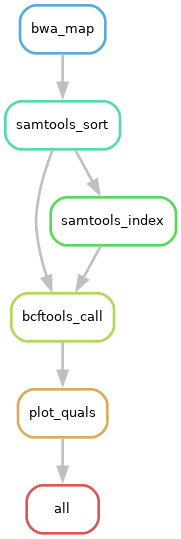
\includegraphics[height=0.5\textheight]{workflows/rulegraph_lifescience.png}
\end{frame}

%%%%%%%%%%%%%%%%%%%%%%%%%%%%%%%%%%%%%%%%%%%%%%%%%%%%%%%%%%%%%%%%%%%%%%%%%%%%%%%%
\begin{frame}[fragile]
  \frametitle{\HandsOn{Produce different Plots}}
  What do you observe, if you try:
  \begin{lstlisting}[language=Bash, style=Shell,basicstyle=\footnotesize]
$ snakemake --rulegraph | dot -Tpng > <your_rulegraph.png>
$ # or
$ snakemake --filegraph | dot -Tpng > <your_filegraph.png>
$ # or
$ snakemake --dag | dot -Tpng > <your_dag.png>
$ # or --dag again after
$ snakemake --delete-all-output -c1
  \end{lstlisting}
\end{frame}

%%%%%%%%%%%%%%%%%%%%%%%%%%%%%%%%%%%%%%%%%%%%%%%%%%%%%%%%%%%%%%%%%%%%%%%%%%%%%%%%
\begin{frame}[fragile]
 \frametitle{Plot Comparison}
 \begin{figure}
  \centering
  \subfloat[\centering \altverb{--rulegraph}]{{ 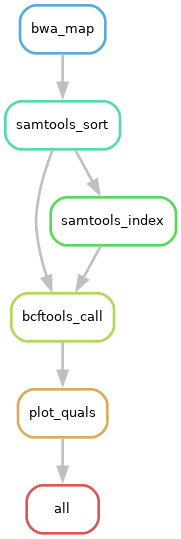
\includegraphics[width=0.2\textwidth, height=0.5\textheight]{workflows/rulegraph_lifescience.png} }}
  \subfloat[\centering \altverb{--filegraph}]{{ 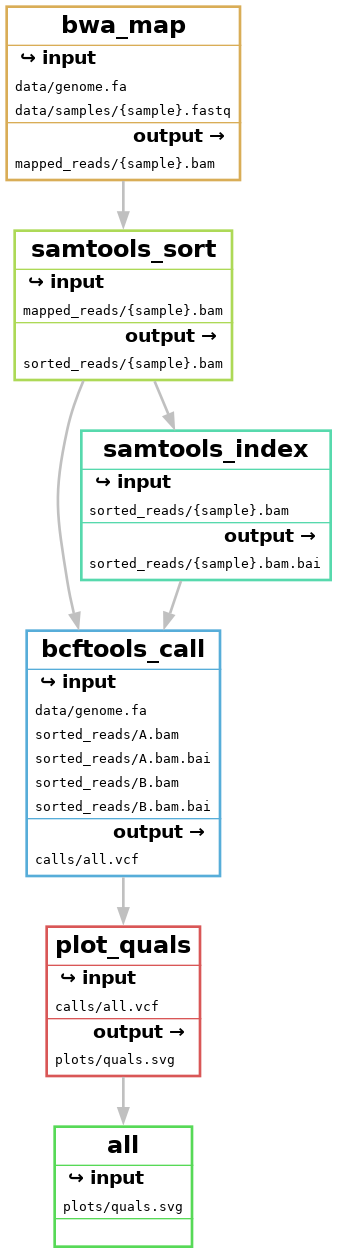
\includegraphics[width=0.2\textwidth, height=0.5\textheight]{workflows/filegraph_lifescience.png} }}
  \subfloat[\centering \altverb{--dag}, with rules done]{{ 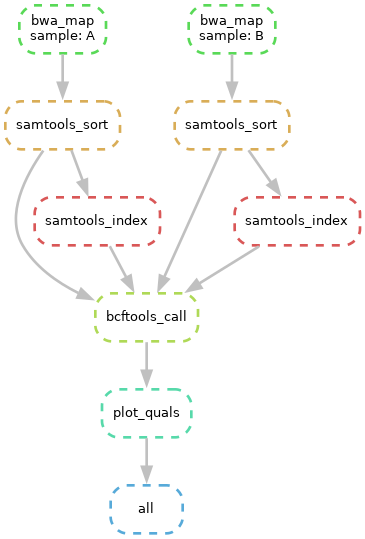
\includegraphics[width=0.2\textwidth, height=0.5\textheight]{workflows/dag_lifescience.png} }}
  \subfloat[\centering \altverb{--dag}, with rules still to do]{{ 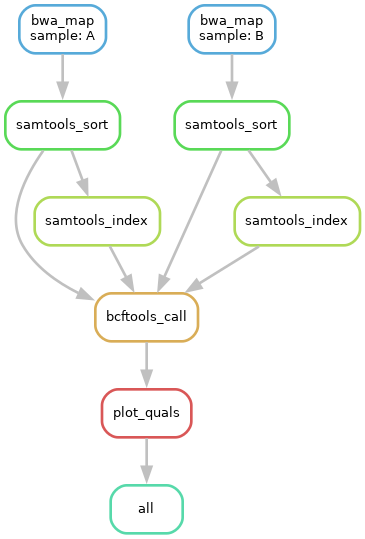
\includegraphics[width=0.2\textwidth, height=0.5\textheight]{workflows/dag_full_lifescience.png} }}
\end{figure}

\end{frame}




